% =========================================================
% Artículo Científico - TPI Algoritmos Genéticos
% =========================================================
\documentclass[12pt,a4paper,twocolumn]{article}

\usepackage[T1]{fontenc}
\usepackage[utf8]{inputenc}
\usepackage[spanish,es-nodecimaldot]{babel}
\usepackage{mathptmx}
\usepackage[margin=2.5cm]{geometry}
\usepackage{amsmath}
\usepackage{graphicx}
\PassOptionsToPackage{hyphens}{url}
\usepackage{hyperref}

\setlength{\columnsep}{1cm}
\pagestyle{empty}

% Estilos para las secciones según el reglamento
\makeatletter
\renewcommand{\section}{\@startsection{section}{1}{\z@}%
  {-2ex \@plus -1ex \@minus -.2ex}%
  {1ex \@plus.2ex}%
  {\fontsize{12}{14}\selectfont\bfseries}}
\makeatother

% Sin numeración en las secciones
\setcounter{secnumdepth}{0}

\begin{document}

\twocolumn[
  \begin{center}
    % Título (Times New Roman, 16, negrita)
    {\fontsize{16}{19}\selectfont\bfseries Optimización mediante Algoritmos Genéticos de la asignación y el balance de carga de alertas de seguridad en Centros de Operaciones de Seguridad (SOC)\par}
    \ifdefined\anonymousversion
    \vspace{1.5em}
    \else
    \vspace{1em}
    % Autores (Times New Roman, 14, negrita)
    {\fontsize{14}{17}\selectfont\bfseries Chacón, A.; Gomez Manna, J.; Tabini, A.; Carloni, N.I.; Mierez, J.\par}
    \vspace{0.5em}
    % Institución (Times New Roman, 12, negrita, cursiva)
    {\fontsize{12}{14}\selectfont\bfseries\itshape Universidad Tecnológica Nacional, Facultad Regional Rosario\par}
    \vspace{1.5em}
    \fi
  \end{center}
]

% =========================================================
% Abstract
% =========================================================
\noindent {\fontsize{10}{12}\selectfont\bfseries Abstract} \\
{\fontsize{10}{12}\selectfont\itshape 
El presente trabajo aborda el desafío del scheduling y asignación de alertas en un Centro de Operaciones de Seguridad (SOC) empleando un Algoritmo Genético Canónico. El volumen masivo de alertas de seguridad excede frecuentemente la capacidad humana, derivando en sobrecarga, fatiga de alertas y potenciales brechas en los Acuerdos de Nivel de Servicio (SLA) para incidentes críticos. Para resolver este problema de optimización combinatoria bajo restricciones, se desarrolló una estrategia evolutiva enfocada en minimizar simultáneamente el tiempo total de resolución, los tiempos de espera y el desbalance de carga entre un número finito de analistas. La metodología propuesta valida empíricamente el algoritmo utilizando una muestra de datos reales derivados del dataset público CICIDS2017 y compara sus resultados operativos con una asignación Round-Robin. La comparación considera espera crítica, backlog y desbalance de carga, métricas directamente relacionadas con la operación del SOC.\par}
\vspace{0.8em}

% =========================================================
% Palabras Clave
% =========================================================
\noindent {\fontsize{10}{12}\selectfont\bfseries Palabras Clave} \\
{\fontsize{10}{12}\selectfont
Algoritmos Genéticos, Centro de Operaciones de Seguridad (SOC), Scheduling, Asignación de Tareas, Balance de Carga, CICIDS2017.\par}
\vspace{1em}

% =========================================================
% Introducción
% =========================================================
\section{Introducción}
Los Centros de Operaciones de Seguridad (SOC) reciben un volumen de alertas que crece con mayor velocidad que la disponibilidad de analistas capacitados para atenderlas. La experiencia y la literatura especializada coinciden en que la sobrecarga (\textit{alert overload}) es uno de los problemas estructurales más persistentes de la operación de un SOC, ya que obliga a decidir con información incompleta y bajo presión de tiempo qué atender primero.

Esa sobrecarga tiene un correlato humano bien documentado en la industria: la fatiga de alertas (\textit{alert fatigue}). Un relevamiento sistemático reciente informa que la mayoría de las organizaciones recibe más de 10.000 alertas diarias y que más del 50\% son falsos positivos [3]. En este contexto, los analistas pueden llegar a ignorar alertas, desactivarlas o delegarlas a colegas, en lugar de investigarlas [3]. La fatiga degrada la calidad de las decisiones de triaje, incrementa el tiempo de respuesta y favorece la rotación del personal capacitado. El resultado es un ciclo que se retroalimenta: más alertas, analistas menos efectivos y tiempos de respuesta más largos, con el agravante de que la demora en atender una alerta de alta severidad incrementa el riesgo de que una intrusión progrese sin ser contenida.

A esta escasez estructural se suma un problema de coordinación: aun cuando el equipo de analistas es suficiente en promedio, la forma en que las alertas se reparten entre ellos rara vez es óptima. Las prácticas habituales de asignación ---turnos fijos, reglas estáticas por tipo de alerta o asignación manual según disponibilidad aparente--- no consideran de forma simultánea la prioridad de cada alerta, el plazo de resolución comprometido (SLA), el tiempo estimado que insumirá resolverla y la carga ya acumulada por cada analista. El resultado observado en la práctica es un desbalance de carga: algunos analistas acumulan \textit{backlog} mientras otros permanecen subutilizados.

El problema fundamental es que la asignación manual no logra minimizar simultáneamente el tiempo total de resolución, los tiempos de espera de las alertas críticas y el desbalance de carga. Por ello, la presente investigación propone diseñar, implementar y evaluar un modelo de Algoritmo Genético Canónico (AG) que distribuya las alertas ---caracterizadas por su prioridad, severidad, tiempo estimado de resolución y SLA--- entre un número limitado de analistas de forma óptima.

Este planteo se relaciona con la priorización de alertas estudiada por Jalalvand et al. [3], quienes organizan los criterios relevantes en dimensiones asociadas con la alerta, el analista, el activo, la organización y el entorno externo. En particular, su relevamiento destaca la necesidad de combinar criterios técnicos con restricciones de recursos humanos y de tiempo, en lugar de ordenar las alertas únicamente por severidad.

% =========================================================
% Elementos del Trabajo y metodología
% =========================================================
\section{Elementos del Trabajo y metodología}
La metodología propuesta se enmarca en la resolución de problemas de optimización combinatoria (específicamente \textit{Job Shop Scheduling}) mediante el uso de Algoritmos Genéticos Canónicos.

La asignación de tareas con tiempos de procesamiento y recursos limitados puede formalizarse como una variante de \textit{Job Shop Scheduling} (JSP), una clase de problemas NP-hard; cuando los tiempos efectivos presentan incertidumbre, el problema se aproxima al \textit{Stochastic Job Shop Scheduling} (SJSP) [4]. En este trabajo se utiliza una instancia determinista con tiempos estimados, por lo que la referencia al SJSP fundamenta una posible extensión de robustez y no implica que la implementación actual modele fallas o distribuciones estocásticas.

Se diseñó una representación cromosómica específica donde cada individuo (cromosoma) codifica una asignación completa de alertas a analistas. Cada gen representa una alerta, y el alelo contenido indica el analista responsable de resolverla.

Esta codificación directa resulta adecuada para representar la decisión principal del problema ---qué analista recibe cada alerta--- y evita introducir una capa de codificación indirecta. Boukedroun et al. [4] reportan que las codificaciones directas pueden representar el cronograma en la estructura de datos y reducir la necesidad de mecanismos complejos de reparación, criterio que se adopta aquí mediante alelos acotados al conjunto de analistas disponibles.

La función de evaluación o \textit{fitness} fue formulada para buscar el menor impacto temporal y el mayor equilibrio, combinando el tiempo total estimado de resolución con penalizaciones estrictas por:
\begin{itemize}
    \item Tiempos de espera prolongados.
    \item Incumplimiento de SLA (especialmente en alertas críticas).
    \item Desbalance de carga entre los analistas operativos.
\end{itemize}

Formalmente, el algoritmo minimiza una penalización operativa $P$ y transforma su resultado en una aptitud positiva a maximizar:
\begin{equation}
\begin{aligned}
J ={}& 0.10\,\widehat{T} + 0.10\,\widehat{W} + 0.20\,\widehat{W}_c + 0.25\,\widehat{R}_c \\
  &+ 0.10\,\widehat{B}_p + 0.05\,\widehat{B}_m + 0.15\,D + 0.05\,O, \\
f ={}& \frac{1}{1 + J}.
\end{aligned}
\end{equation}
Aquí, las variables con sombrero representan magnitudes normalizadas: $\widehat{T}$ es el makespan relativo al horizonte, $\widehat{W}$ la espera promedio, $\widehat{W}_c$ la espera crítica, $\widehat{R}_c$ el retraso crítico respecto del SLA, $\widehat{B}_p$ el backlog ponderado por prioridad, $\widehat{B}_m$ los minutos de backlog, $D$ el desbalance relativo de carga y $O$ la sobrecarga relativa. La configuración oficial utiliza $w_T=0.10$; la ablación comparativa fija $w_T=0$.

El algoritmo evoluciona la población generación tras generación aplicando selección por ranking, cruzamiento para recombinar asignaciones exitosas, mutación por gen y elitismo. La población inicial incluye una solución Round-Robin como referencia y la política de atención dinámica prioriza las alertas disponibles según prioridad, severidad y urgencia del SLA. La selección por torneo y por ruleta se conservan como alternativas reproducibles. Estos operadores forman parte del marco clásico de planes reproductivos y operadores genéticos desarrollado por Holland, que también analiza la robustez de los planes evolutivos y el papel de las codificaciones en sistemas adaptativos [2].

La configuración oficial utiliza una población de $N=50$ individuos y evoluciona durante $G=200$ generaciones, es decir, hasta 10.000 evaluaciones de individuos por corrida. La probabilidad de cruzamiento de un punto es $P_c=0.75$ y la probabilidad de mutación por gen es $P_m=0.05$. Se preservan los tres mejores individuos por generación y se utiliza selección por ranking. Los resultados principales se reportan sobre 20 semillas ($42$--$61$). El grid search de 18 combinaciones se utilizó únicamente como exploración de hiperparámetros, con 15 generaciones por combinación; su mejor configuración ($N=20$, $P_m=0.05$, $P_c=0.60$) no reemplaza la configuración oficial $N=50$, $G=200$.

Para validar empíricamente el modelo, se utilizó una base de datos representativa derivada del dataset público \textbf{CICIDS2017} [1]. A partir de una muestra aleatoria de eventos, se inyectaron sintéticamente atributos operativos (prioridad, severidad, SLA y tiempo estimado de resolución) para simular de forma fiel y rigurosa el flujo de alertas continuo que enfrenta un SOC.

La selección de estos atributos está alineada con la taxonomía de criterios de priorización de Jalalvand et al. [3]: prioridad y severidad representan propiedades de la alerta; el tiempo de resolución aproxima el tiempo disponible y la carga del analista; y el SLA expresa la dimensión organizacional de cumplimiento y oportunidad (\textit{timeliness}). Esta correspondencia ofrece una justificación metodológica para la función de aptitud, aunque los atributos hayan sido generados sintéticamente.

La tabla de alertas derivadas contiene 500 registros: 207 de prioridad Alta, 111 Media, 97 Baja y 85 Crítica. La severidad media es 53.5 y el tiempo estimado medio de resolución es 41.2 minutos. Estos valores describen la instancia concreta sobre la que se comparan las asignaciones y no deben interpretarse como propiedades originales del dataset CICIDS2017.

Como baselines operativos se utilizaron tres reglas deterministas. Round-Robin asigna las alertas secuencialmente entre los analistas, sin considerar carga ni prioridad. Menor carga asigna cada alerta al analista con menor carga acumulada. Urgencia balanceada ordena las alertas por prioridad, severidad y SLA, y asigna cada una al analista con menor carga; por lo tanto, incorpora urgencia sin realizar búsqueda evolutiva. Estas reglas se utilizan como referencias heurísticas y no forman parte del entrenamiento del AG.

% =========================================================
% Resultados
% =========================================================
\section{Resultados}
Las ejecuciones del algoritmo se evaluaron mediante métricas operativas y se compararon con una asignación Round-Robin. Esta comparación permite distinguir la convergencia interna del algoritmo de su impacto efectivo sobre el triaje y la distribución de trabajo.

\begin{figure}[t]
  \centering
  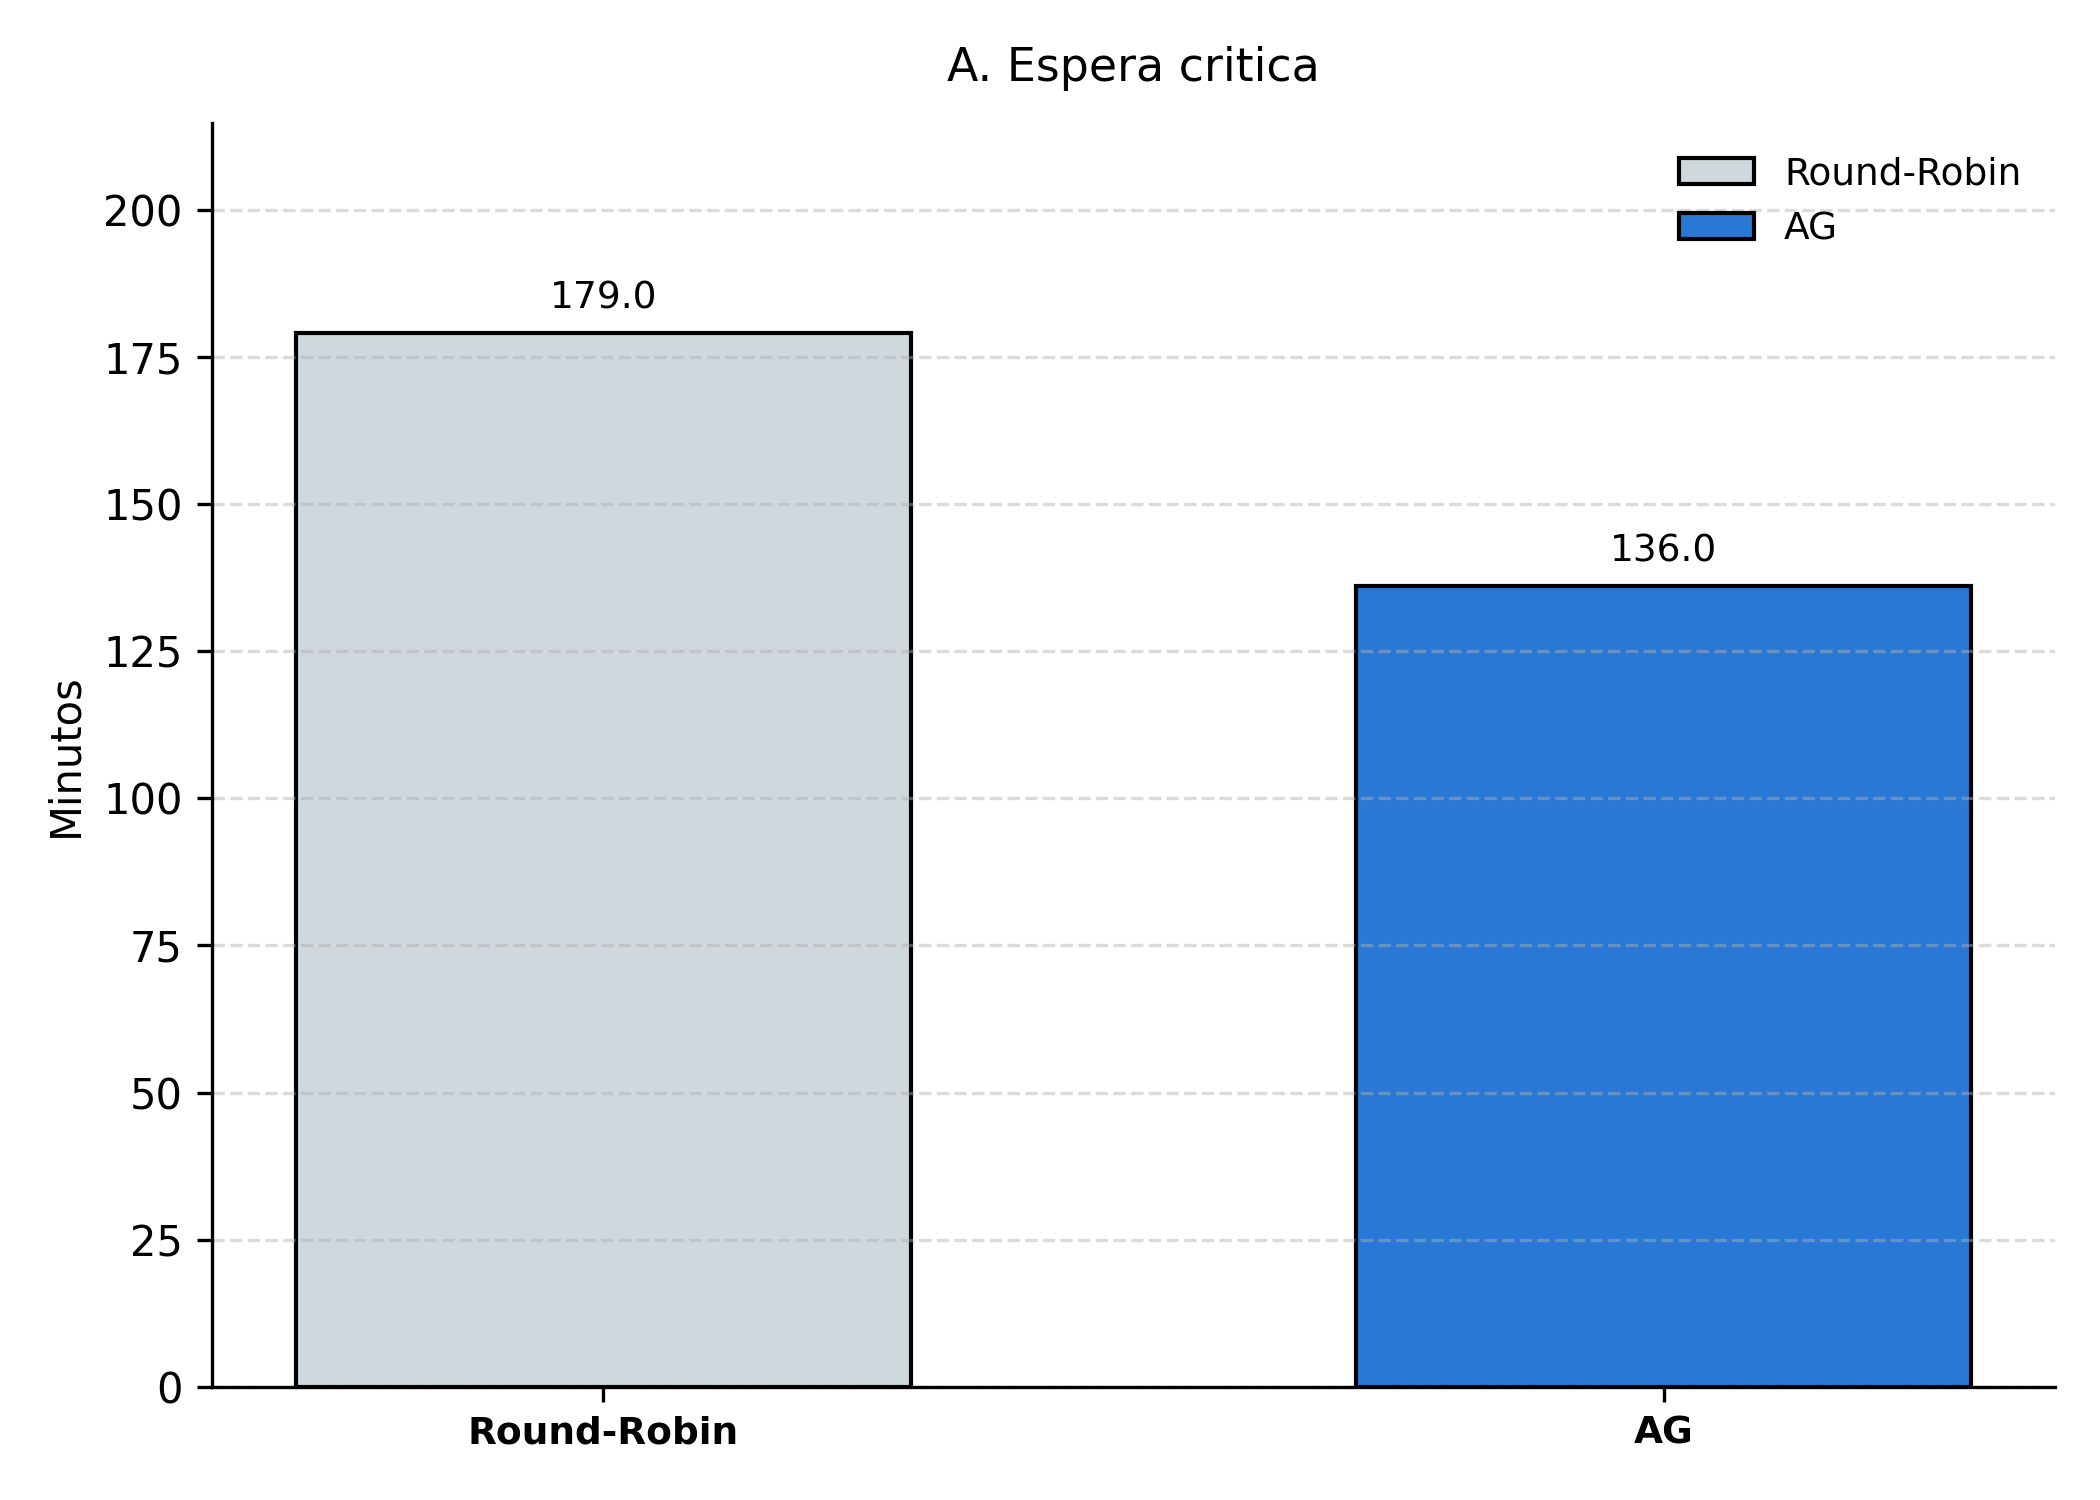
\includegraphics[width=\columnwidth]{../outputs/figures/espera_critica_comparativa.png}
  \caption{Espera crítica promedio para la corrida reproducida con la semilla $42$.}
  \label{fig:comparativa-espera}
\end{figure}

\begin{figure}[t]
  \centering
  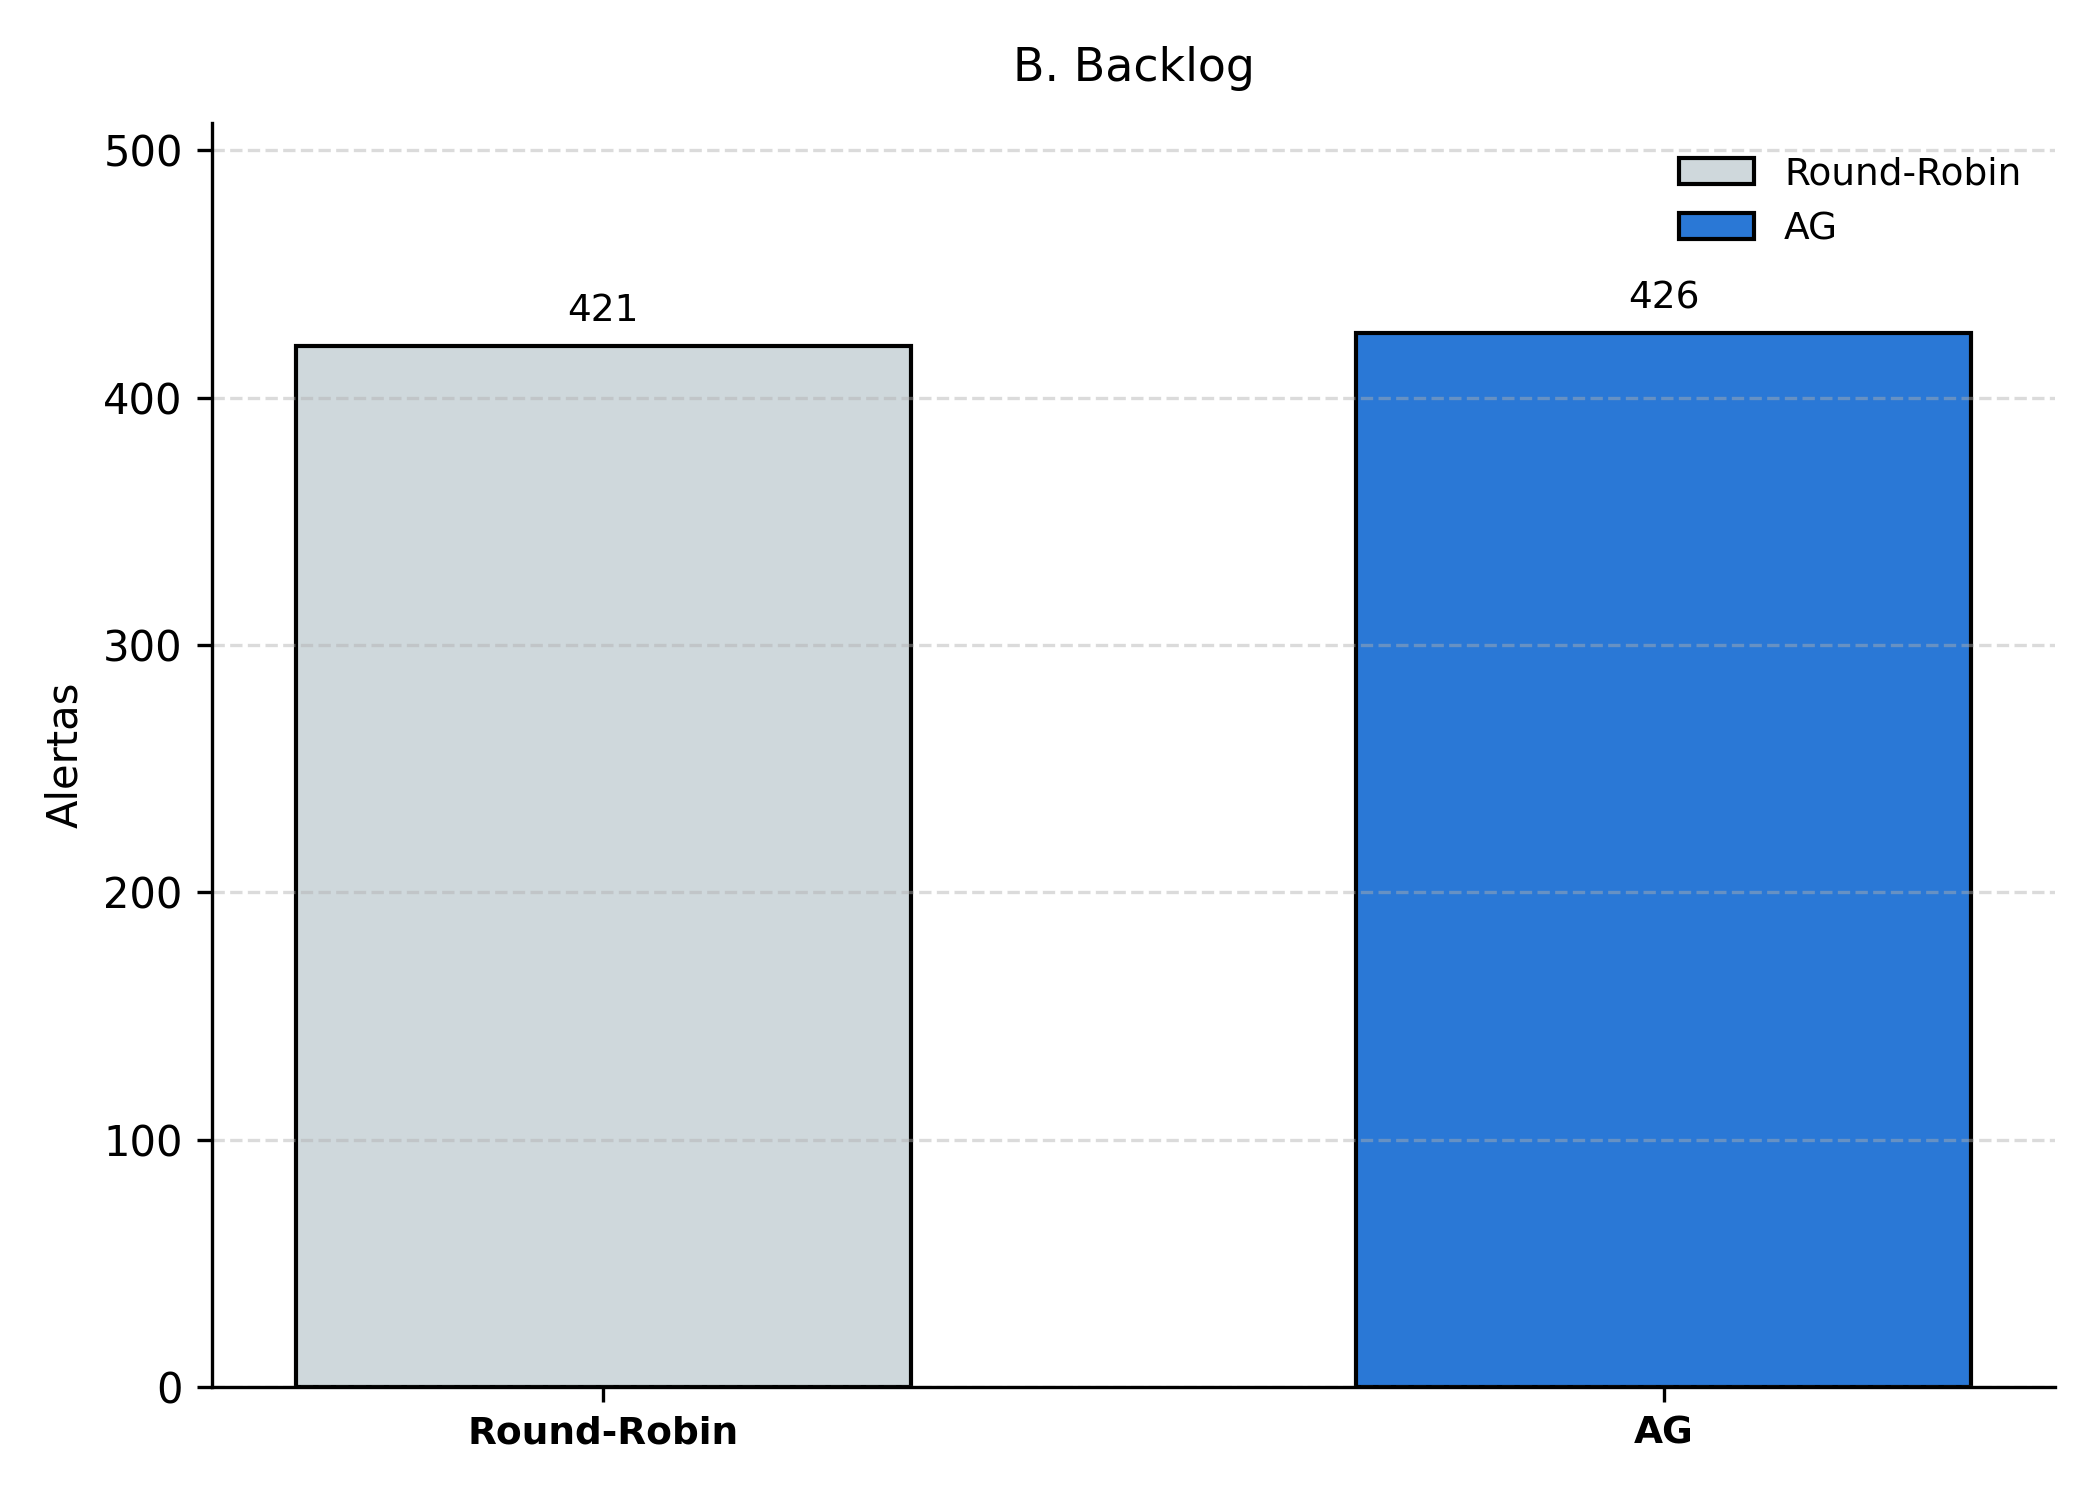
\includegraphics[width=\columnwidth]{../outputs/figures/backlog_comparativa.png}
  \caption{Backlog total para la corrida reproducida con la semilla $42$.}
  \label{fig:comparativa-backlog}
\end{figure}

\begin{figure}[t]
  \centering
  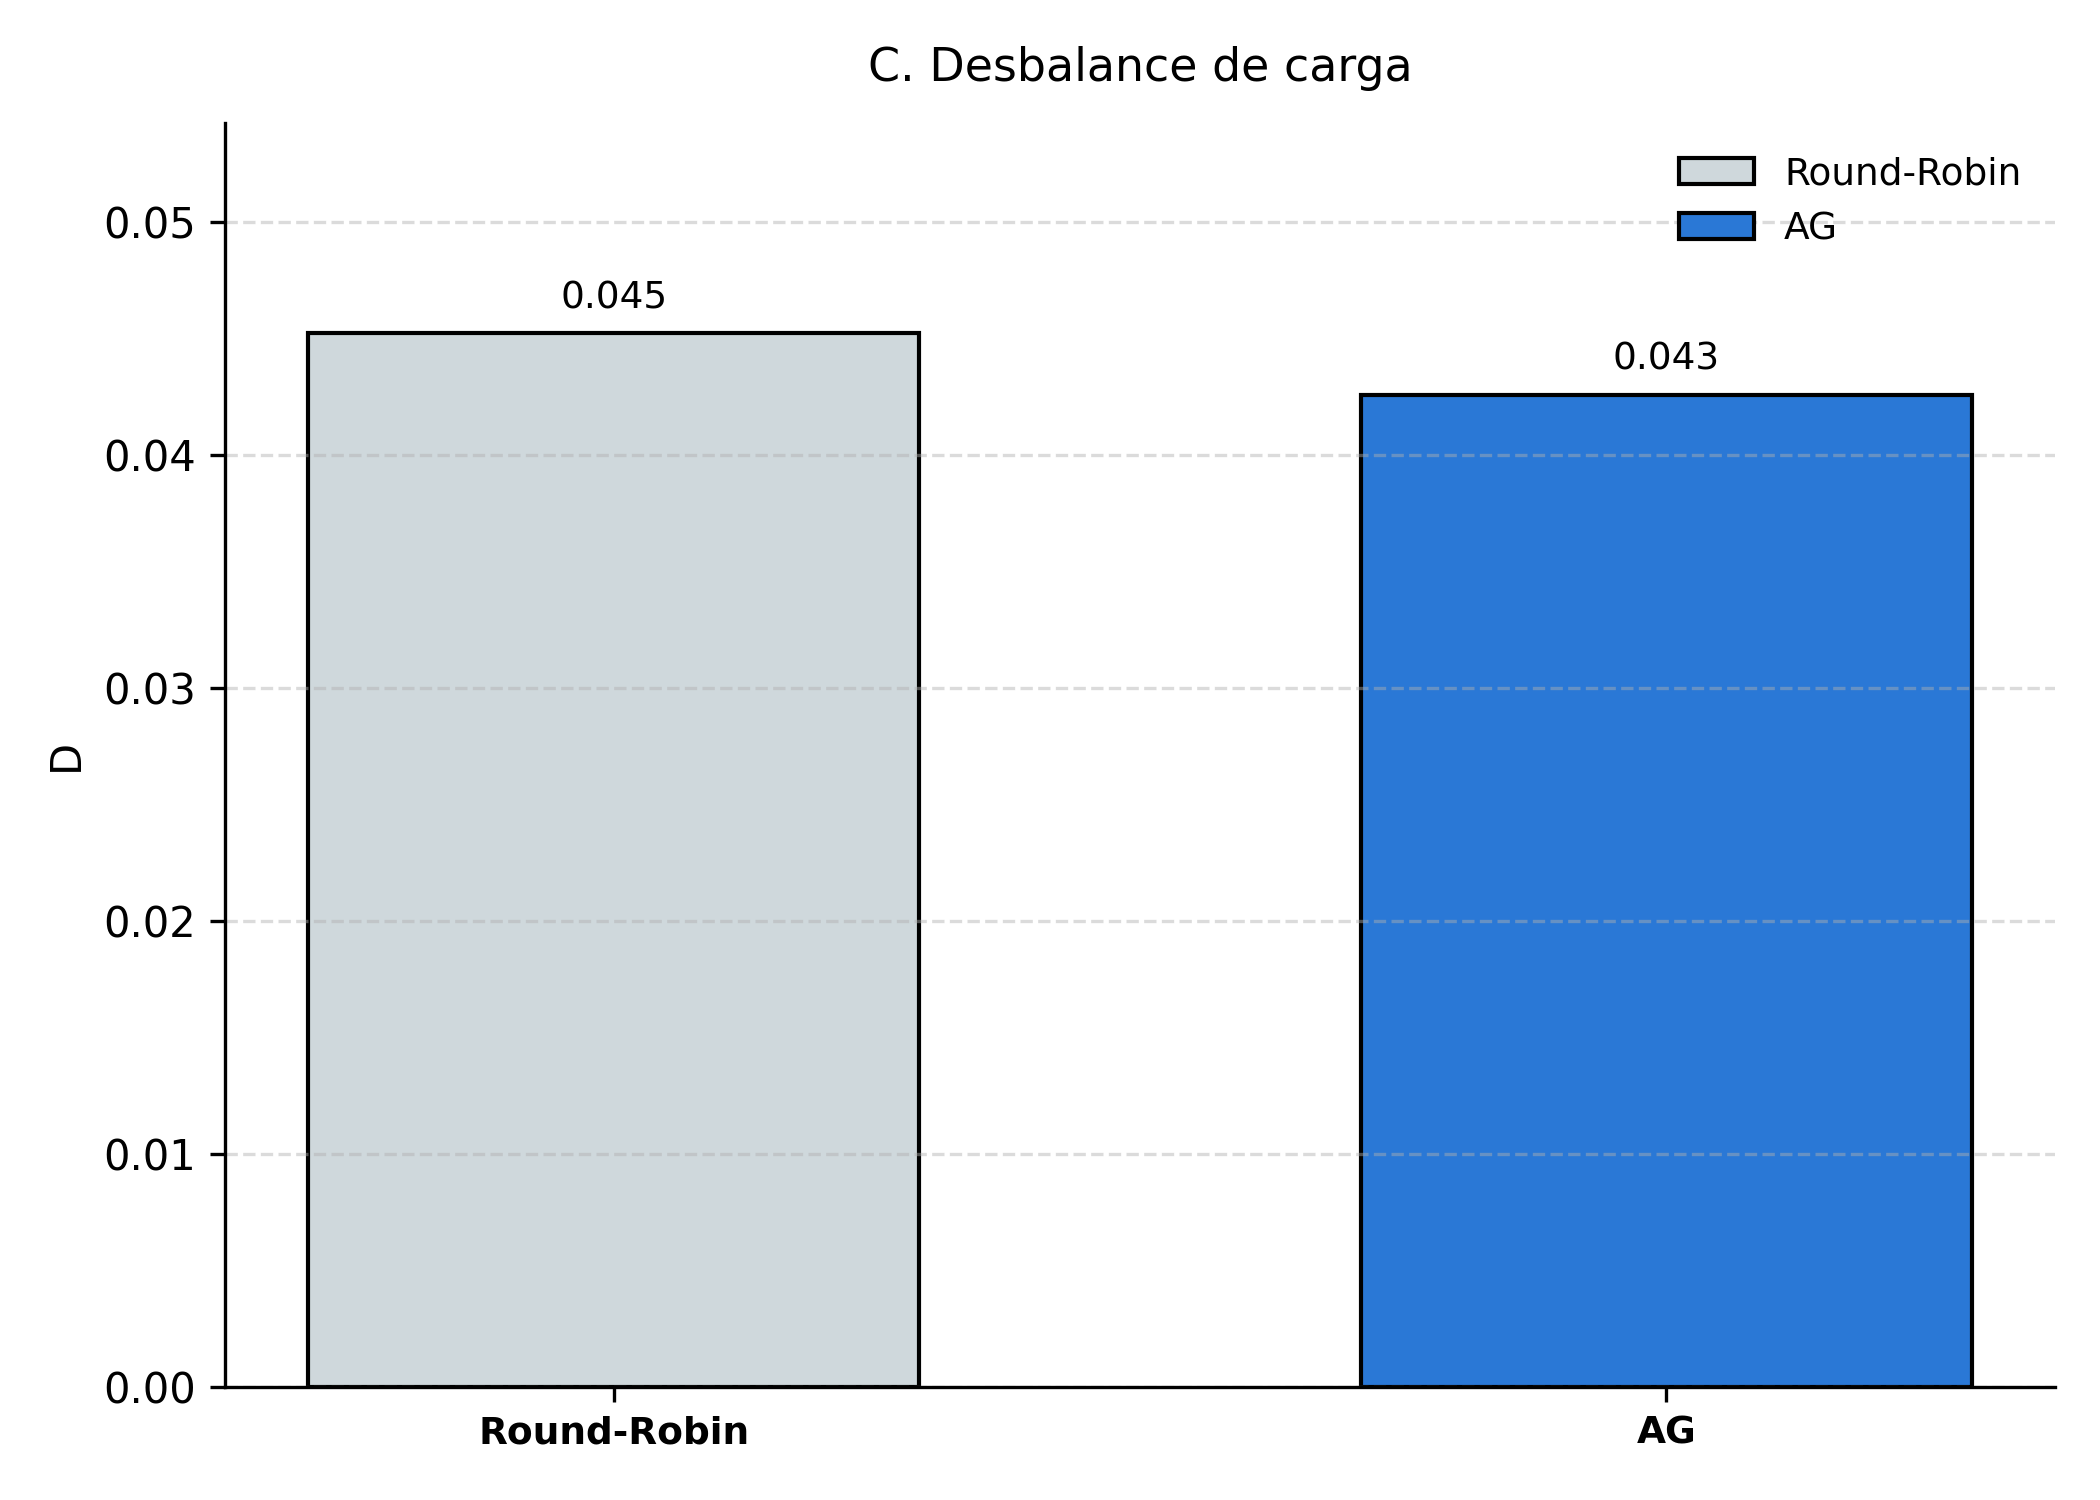
\includegraphics[width=\columnwidth]{../outputs/figures/desbalance_comparativa.png}
  \caption{Desbalance relativo de carga para la corrida reproducida con la semilla $42$.}
  \label{fig:comparativa-desbalance}
\end{figure}

Las Figuras~\ref{fig:comparativa-espera},~\ref{fig:comparativa-backlog} y~\ref{fig:comparativa-desbalance} presentan una corrida puntual (semilla 42), mientras que las cifras agregadas de este párrafo corresponden a 20 semillas. En la corrida de las figuras, la espera crítica del AG fue 136.0 minutos, su backlog 426 alertas y su desbalance $D=0.043$; este último valor es superior a la media, por lo que la semilla 42 no debe tomarse como representativa del balance típico. En el agregado, Round-Robin obtuvo una espera crítica media de 179.0 minutos frente a 136.1 del AG, una mejora media de 24.0\%. El backlog fue de 421 alertas para Round-Robin y 425.1 en promedio para el AG, mientras que el desbalance relativo medio fue $D=0.045$ y $D=0.027$, respectivamente. Por lo tanto, el AG mejora la espera crítica y el balance en promedio, aunque aumenta levemente el backlog; esto evidencia la necesidad de evaluar varias semillas y ajustar la función de aptitud según las prioridades operativas.

La instancia está deliberadamente sobredimensionada respecto del horizonte: 500 alertas con 41.2 minutos medios representan aproximadamente 20.600 minutos-analista de demanda, mientras que 10 analistas durante 480 minutos ofrecen 4.800 minutos-analista de capacidad. La razón demanda/capacidad es, por tanto, cercana a 4.3 y hace inevitable que una fracción elevada de alertas quede fuera del turno. En consecuencia, el backlog total (425.1 para el AG frente a 421 para Round-Robin) es principalmente un efecto estructural de capacidad y no un diferenciador algorítmico fuerte; la composición del backlog por prioridad es la métrica más informativa para evaluar qué riesgos se postergan.

A partir del análisis generacional se observaron además las siguientes medidas:

\begin{itemize}
    \item \textbf{Mejora generacional:} El mejor \textit{fitness} global alcanzó $5.319\times 10^{-1}$. La evaluación sobre 20 semillas produjo una media de $5.282\times 10^{-1}$ y una desviación estándar de $1.71\times 10^{-3}$.
    \item \textbf{Tiempos de espera y de resolución:} La solución global seleccionada alcanzó una espera crítica de 136.1 minutos. En 20 semillas, la espera crítica media fue 136.1 minutos ($\sigma=7.7$). El makespan medio fue 2138.4 minutos con el peso oficial $w_T=0.10$, frente a 2180.4 minutos en la ablación $w_T=0$; la diferencia pareada de 42.0 minutos, equivalente a aproximadamente $1.9\%$ del makespan de la ablación, fue significativa ($p=8.2\times10^{-5}$). Por su magnitud, se interpreta como una mejora temporal modesta pero consistente, no como una reducción operativa drástica.
    \item \textbf{Desbalance y Backlog:} El desbalance medio fue $D=0.0271$ y el backlog medio 425.05 alertas. En la ablación sin makespan, el desbalance fue $D=0.0308$ y el backlog 425.20; las diferencias de desbalance ($p=0.189$) y backlog total ($p=0.832$) no fueron significativas.
    \item \textbf{Eficiencia computacional:} La corrida oficial realizó 10.000 evaluaciones y tomó 34.9 segundos dentro del motor, con una medición externa de 36.4 segundos por semilla. Este costo es compatible con reevaluaciones por lote, aunque no corresponde describirlo como una ejecución de milisegundos.
\end{itemize}

El archivo de distribución final muestra las cargas asignadas de la corrida oficial. En el grid search de 18 configuraciones, la mejor aptitud fue obtenida con población 20, mutación 0.05 y cruzamiento 0.60. Además, la comparación de baselines mostró que la regla de urgencia balanceada puede distribuir mejor la carga, mientras que el AG obtiene una espera crítica menor. Este resultado refuerza que no existe dominancia simultánea en todas las métricas.

El backlog por prioridad debe interpretarse junto con la ablación: al quitar el makespan, el backlog de Alta aumenta de 203.55 a 205.85 alertas, mientras que el backlog de Crítica disminuye de 34.15 a 31.95. Es decir, la configuración sin makespan protege mejor las alertas críticas, pero desplaza parte del costo hacia las alertas Alta.

Para controlar el riesgo de falsos positivos por comparaciones múltiples, se aplicó la corrección de Bonferroni a las cinco pruebas pareadas entre la configuración oficial y la ablación: espera crítica, desbalance, backlog total, backlog ponderado y makespan. El nivel ajustado fue $\alpha=0.01$. Tras la corrección, la diferencia en espera crítica ($p_{aj}=9.5\times10^{-6}$) y makespan ($p_{aj}=4.1\times10^{-4}$) permanecieron significativas; las diferencias en desbalance ($p_{aj}=0.947$), backlog total ($p_{aj}=1.000$) y backlog ponderado ($p_{aj}=0.121$) no alcanzaron significancia. Esta corrección se reporta para distinguir efectos robustos de resultados exploratorios.

% =========================================================
% Discusión
% =========================================================
\section{Discusión}
Los resultados obtenidos confirman que la formulación de una función de aptitud multifactorial (que penalice simultáneamente tiempos muertos y desbalance de carga) es eficaz para superar las limitaciones de las heurísticas de asignación convencionales (tales como turnos fijos o reglas \textit{First-In-First-Out}). 

A diferencia de los enfoques estáticos manuales, el Algoritmo Genético permite expresar en una única función objetivo el tiempo de resolución, la espera crítica, el backlog y el balance de carga. Sin embargo, la comparación de esta corrida no muestra una superioridad automática frente a Round-Robin en todas las métricas. Esto es consistente con la observación de Jalalvand et al. [3] de que los métodos de optimización permiten incorporar explícitamente restricciones como la disponibilidad de analistas y el tiempo de investigación, aunque permanecen menos explorados que los enfoques basados en aprendizaje automático. En consecuencia, el modelo propuesto se interpreta como una forma de Alert Prioritisation (AP) automatizada para el triaje y la asignación inicial, no como un reemplazo de la validación experta ante incidentes nuevos o ambiguos.

El backlog total no debe leerse como una medida aislada de calidad del algoritmo en esta instancia: la demanda estimada supera 4.3 veces la capacidad del turno. La comparación relevante es qué prioridades se preservan dentro de ese desborde: el AG reduce la espera crítica y la cantidad de alertas críticas pendientes, aun cuando posterga una fracción adicional de alertas de prioridad Alta. Esta lectura distingue una limitación estructural de capacidad de una decisión de priorización.

El costo computacional, cercano a 35 segundos por semilla, permite reevaluaciones por lote, aunque no una respuesta instantánea por alerta individual. La ablación pareada muestra que el peso del makespan reduce significativamente el tiempo total de finalización, pero solo en una magnitud relativa cercana al $1.9\%$ y sin modificar significativamente el desbalance. Por ello, el makespan debe interpretarse como una restricción temporal operacional modesta y consistente, no como la causa exclusiva del balance observado. La literatura de scheduling también vincula la reducción y estabilización del tiempo crítico de procesamiento con una mayor robustez frente a perturbaciones [4].

% =========================================================
% Conclusión
% =========================================================
\section{Conclusión}
El presente trabajo demuestra empíricamente la viabilidad de utilizar Algoritmos Genéticos Canónicos para abordar el problema de asignación de alertas en un SOC. Se logró modelar una representación cromosómica y una función de evaluación que integran tiempo de resolución, espera crítica, backlog y balance de carga. Al validar el modelo sobre una muestra adaptada del dataset CICIDS2017 y compararlo con Round-Robin, el AG mejora significativamente la espera crítica y el desbalance, con un costo acotado en backlog total. La comparación pareada con una ablación del makespan muestra además que dicho término reduce significativamente el tiempo total de finalización, pero no explica por sí solo la mejora del balance.

Como líneas de trabajo futuro, se propone avanzar desde la automatización hacia una colaboración Humano--IA: los analistas podrían revisar las asignaciones y ajustar dinámicamente los pesos de las penalizaciones mediante retroalimentación activa, actualizando la función de aptitud según el contexto operativo. También se incorporarán atributos de los activos afectados ---por ejemplo, criticidad, vulnerabilidad o dependencia--- dentro de la representación genética, y se evaluará la robustez del cronograma frente a variaciones estocásticas en los tiempos de resolución. Estas extensiones responden a las brechas identificadas por Jalalvand et al. [3] y a la perspectiva de robustez del SJSP estudiada por Boukedroun et al. [4].

% =========================================================
% Agradecimientos
% =========================================================
\section{Agradecimientos}
{\fontsize{10}{12}\selectfont
A la cátedra de Algoritmos Genéticos por el marco metodológico, orientación técnica y soporte brindado para el desarrollo integral de la presente investigación.
\par}

% =========================================================
% Referencias
% =========================================================
\section{Referencias}
{\fontsize{10}{12}\selectfont
\noindent [1] Sharafaldin, I., Lashkari, A. H., y Ghorbani, A. A. (2018). \textit{Toward Generating a New Intrusion Detection Dataset and Intrusion Traffic Characterization}. CICIDS2017.

\noindent [2] Holland, J. H. (1992). \textit{Adaptation in Natural and Artificial Systems}. MIT Press.

\noindent [3] Jalalvand, F., Chhetri, M. B., Nepal, S., y Paris, C. (2024). \textit{Alert Prioritisation in Security Operations Centres: A Systematic Survey on Criteria and Methods}. ACM Computing Surveys, 57(2), 1--36. https://doi.org/10.1145/3695462

\noindent [4] Boukedroun, M., Duvivier, D., Ait-el-Cadi, A., Poirriez, V., y Abbas, M. (2023). \textit{A hybrid genetic algorithm for stochastic job-shop scheduling problems}. RAIRO--Operations Research, 57(4), 1617--1645. https://doi.org/10.1051/ro/2023067
\par}

\vspace{1.5em}

\ifdefined\anonymousversion
\else
% =========================================================
% Datos de Contacto
% =========================================================
\noindent {\fontsize{10}{12}\selectfont\bfseries Datos de Contacto:}\\
{\fontsize{10}{12}\selectfont\itshape 
Chacón, A.; Gomez Manna, J.; Tabini, A.; Carloni, N.I.; Mierez, J. Universidad Tecnológica Nacional, Facultad Regional Rosario. Zeballos 1341, Rosario, Santa Fe. E-mail: alumnos@utn.edu.ar.
\par}
\fi

\end{document}
